% !TEX root = thesis.tex
% !TEX program = pdflatex
% !TEX bibprogram = biber

% se la bibliografia non va: pdflatex thesis, biber thesis, pdflatex thesis

% toptesti document class
\documentclass[
    a4paper,
    corpo=12pt,
    twoside,
    stile=standard,
    %evenboxes,
    tipotesi=triennale,
    numerazioneromana,
    openright, 
    printing,
    cucitura=7mm,
    %dvipsnames,
]{toptesi}

\input{common/packages}

\input{common/package_config}

\input{common/new_commands}

\newcommand{\thesistitle}{Permutation flowshop scheduling with periodic maintenance}
%\newcommand{\thesissubtitle}{Eventuale sottotitolo} % not strictly necessary, leave empty if not needed
\newcommand{\thesiscandidatename}{Dania}
\newcommand{\thesiscandidatesurname}{Ottenga}
\newcommand{\thesissupervisoronename}{Fabio}
\newcommand{\thesissupervisoronesurname}{Salassa}
\newcommand{\thesisdate}{July 2026}
\newcommand{\thesiscourse}{Bachelor degree in Management Engineering}
\newcommand{\academicYear}{A.a. 2025/2026}
\newcommand{\thesisuniversity}{Politecnico di Torino}
\newcommand{\thesiscandidatetext}{Candidate}
\newcommand{\thesissupervisortext}{Supervisor}

\input{common/font_config.tex}

\addbibresource{bibliography.bib}

% to load the glossaries, not needed if using bib2gls
\input{glossaries.tex}
\makeglossaries

\begin{document}

\input{common/config}

\input{common/toptesi_config}

\english

% front page -- add your info in common/thesis_info.tex
\input{common/frontpage.tex} % new frontespizio (2023)
%\retrofrontespizio
% insert text for the back of the front page
% if you insert any remove the following \paginavuota
% either a blank page or a back is needed to have double-sided printing
% pay attention to leave the space for the page

\frontmatter % not strictly needed, as toptesi takes care of it already

%DA AGGIUNGERE PER STAMPA
% paginavuota
% abstract if needed
% \begin{abstract}
%     \input{content/abstract.tex}
% \end{abstract}

% to create blank pages for openright in frontmatter
% use one of the following two methods
% 1) use the following three lines
%\phantom{0} % needed otherwise cleardoublepage does not clean the page because it sees it empty
%\cleardoublepage
%\thispagestyle{empty} % to have empty page, without numbers
% 2) or

% summary (uncomment until "end summary" if needed)
%\sommario
%\input{content/summary}

%\phantom{0}
%\cleardoublepage
%\thispagestyle{empty}
% end summary

%\ringraziamenti % acknowledgements
%\input{content/acknowledgements}

\paginavuota

\tableofcontents

% actually abbreviation is the name used for acronym in glossaries-extra
% title sets the name
% type tells the type of glossary to print
% style overrides the global style
% here we are printing only abbreviations
% printunsrtglossary if using record, otherwise printglossary is ok
%\paginavuota
%\printunsrtglossary[style=altlist,title=Glossario,type=\glsxtrabbrvtype]

% also list of symbols here if needed

\input{common/post_summary_config.tex}

\mainmatter

%\part{Prima Parte} % parts division, not needed
% Chapters always open on a right-side page, i.e. odd numbers, so a blank page is inserted if needed
%\cleardoublepage[empty] % to have a fully blank page
% a blank page appears before the first chapter in some configurations, on the last version it doesn't

% chapters go here
\chapter{Introduction to combinatorial optimization}

\label{sec:intro_comb_opt}

\textbf{Combinatorial Optimization} (CO) is the search for a ``best'' configuration of a set of discrete variables to achieve some goals in a typically finite domain. To optimize means to minimize or maximize the objective function, respecting the constraints. The solution will be a combination of variables, present in the set of all feasible assignments: the search (or solution) space. 

A CO problem is defined by:
\begin{itemize}
    \item \textbf{Set of variables:} $V = \{x_1, x_2, \dots, x_n\}$.
    \item \textbf{Variable domains:} $D = \{D_1, D_2, \dots, D_n\}$ where $x_i$ can take on values ($x_i \in D_i$).
    \item \textbf{Constraints among variables:} $\Omega$ is the set of restrictions that limits all the possible combinations of values defining the solution space $S \subseteq D_1 \times \dots \times D_n$.
    \item \textbf{Objective function:} $f: S \rightarrow \mathbb{R}$ assigns a numeric value to each admissible configuration.
\end{itemize}

\section[Historical roots]{Historical roots}

The origins of CO lie in economic problems: the planning and management of operations and the efficient use of resources. It was initially conceived by Kantorovich and Koopmans and was motivated by applications in transportation and transshipment \cite{SCHRIJVER20051}. Soon more technical applications were developed and today we see discrete optimization problems everywhere: portfolio selection, capital budgeting, design of marketing campaigns, investment planning and facility location, political districting, gene sequencing, classification of plants and animals, the design of new molecules, the determination of ground states, layout of survivable and cost-efficient communication networks, positioning of satellites, sizing of truck fleets, layout of mass transportation systems and scheduling of buses and trains, assignment of workers to jobs such as drivers to buses and airline crew scheduling, design of unbreakable codes, etc. The list of applications is endless; even in areas like sports, archaeology or psychology \cite{grotschel1995combinatorial}.

\section[Families of problems]{Families of problems}

We can divide the CO in five macro-groups: \textbf{the assignment problems} that aim to find the permutation where the sum of the costs of all the variables is the smallest possible by assigning a task to each agent; \textbf{the transportation problems} that aim to minimize the cost of transporting a product between several sources and destinations, \textbf{the packing/covering problems} that aim to minimize the number of containers used or the value of the object inserted in them; \textbf{the traveling salesman problems} that aim to find the order of the given places that the salesman must visit (each location exactly once) traversing the shortest route and \textbf{the scheduling problems} that aim to allocate resources to perform a set of tasks over a specific period minimizing the completion time.

\section{Complexity and Solving Strategies}

The main challenge in CO is the size of the search space $S$. For many problems, $S$ grows factorially or exponentially with the number of variables $n$.

\subsection{NP-hard Problems}

Visiting all the possibilities in our search space to find the best one is not always computationally possible; these are known as \textbf{NP-hard problems} for which no polynomial time algorithm is currently known. This means that as the problem size increases, the time required to find the "best" configuration using exact methods becomes practically impossible, even for modern computers \cite{blum2003metaheuristics}. 

\subsection{Heuristics and Metaheuristics}

In these cases, we can rely on algorithms that produce an approximately optimal solution by making a trade-off between computational time and solution quality. So, the aim is to find the one solution that is close to the optimal in a reasonable time \cite{paschos2009overview}.

Approximate algorithms are divided into two major categories of algorithms. \textbf{Heuristics} are problem-specific algorithms designed to find a good solution quickly. They often follow a greedy approach (e.g., in the traveling salesman problem, always moving to the nearest unvisited city). While fast, heuristics often get stuck in local optima - solutions that are better than their neighbors but worse than the global best. On the other hand, \textbf{Metaheuristics} are higher-level frameworks that orchestrate one or more heuristics to explore the search space more efficiently. Unlike simple heuristics, metaheuristics include mechanisms to escape local optima (e.g., by allowing temporary "worse`` moves or maintaining a population of solutions). Common examples include Genetic Algorithms, Simulated Annealing, and Ant Colony Optimization.

\chapter{Introduction to Machine Scheduling}
\label{sec:intro_proj_sch}

\textbf{Machine Scheduling} aims to perform a number of jobs, each of which consists of a sequence of operations, by using a number of machines. To complete a job, each of its operations must be processed in the order given by the sequence. The processing of an operation requires a use of a particular machine for a given duration, the processing time. The objective is to find a processing order to minimize the makespan.

A distinction can be made between sequences and schedules. A \textbf{sequence} corresponds to an ordering of the operations on each machine that allows the sequence of the operations corresponding to each job. Corresponding to each sequence there is an infinity of feasible \textbf{schedules} obtained by specifying the exact starting and finishing time of each operation. A schedule determines for each job a \textbf{completion time} in which its last operation is finished \cite{kan2012machine}.

\section[Problem classification]{Problem classification}

To classify the various types of machine scheduling problems, the three field notation introduced by \textbf{Graham} is used \cite{10.1145/3431232} \cite{weglarz2012project}:
\begin{itemize}
    \item $\boldsymbol{\alpha}$ for the \textbf{resources}: we can consider a single machine, parallel identical machines, or flow shop environments.
    \item $\boldsymbol{\beta}$ for the \textbf{properties of tasks}: where we can consider:
    \begin{itemize}
        \item \textbf{Preemption}: not allowed (one cannot stop the task once it has started).
        \item \textbf{Precedence}: no constraints, strict constraints (finish-start: the successor cannot start before the predecessor finishes) and generalized constraints.
        \item \textbf{Deadlines}: not assumed, imposed on activities and imposed on the project.
    \end{itemize}
    \item $\boldsymbol{\gamma}$ for the \textbf{criterion} (the objective function) which is to minimize the makespan ($C_{\text{max}}$), or the completion time of the last job.
\end{itemize}

\section[Flow shop scheduling]{Flow shop scheduling}

\textbf{Flow Shop} is a processing system in which the task sequence of each job is fully specified (chain precedence) and all the jobs visit the work stations in the same order. In a pure flow shop each job visits all stages but more generically can have fewer tasks and can skip some stations. But it's assumed that a job visiting a $i' > i$ station cannot go back to the previous one (\textit{i}). There is also another case: the reentrant flow shop. Here jobs can recycle back and be reprocessed at the same station, or sequence of stations, multiple times.

There are many variations to the general flow shop like the \textbf{simple flow shop}. Here we can make these considerations: each stage can handle one operation at a time, each task of a job requires a different machine, all jobs are available simultaneously at the start and remain available until the work is finished, each job can be in one place at the time, no preemption is allowed, when a job is finished in one machine, it's immediately available for the next one so there are no delays due to setups or transfer, intermediate storage between machines is unlimited. Then there is the \textbf{general job shop}, which is described exactly like the simple flow shop but the machine sequence of different jobs may differ, and the \textbf{hybrid (compound or flexible) flow shop} where work station may consists in several functionally identical processors in parallel \cite{emmons2012flow}.

\section[Permutation Flow Shop (PFSSP)]{Permutation Flow Shop (PFSSP)}

The \textbf{Permutation Flow Shop Scheduling Problem} (PFSSP) consists of a set of jobs on a set of machines with the objective of minimizing the makespan. Each job can be processed on one machine at a time and each machine can process one job at a time and the operations can't be preemptable. The sequence in which the jobs are to be processed is the same for each machine.

The PFSSP problem is denoted by the symbols $n/m/P/C_{\text{max}}$ where $n$ represents the number of jobs, $m$ the number of machines, $P$ is the processing time and $C_{\text{max}}$ is the makespan. Based on the considerations exposed, the \textbf{PFSSP} model will be used for the case study analysis \cite{LI20121921}.
\chapter{Problem identification}
\label{sec:intro_prob_id}

The problem addressed in this study takes into consideration a permutation flowshop scheduling with periodic maintenance. The aim is, given the number of jobs, the number of machines and the processing time of every job on every machine, to minimize the completion time of the final job in the sequence. The production will be carried out within working shifts. To reduce time wasting given by the transfer of duties and the explanation of the work carried out up to the end of the shift, we will consider the end of the shift as a time limit to finish the job we've started so there are no jobs that start in a shift and end in another. So when deciding whether to start a job during we see that there isn't enough time to complete the job in the current shift, we will wait and start producing it in the next one.

\section[Mathematical Notation: Parameters, Indexes and Variables]{Mathematical Notation: Parameters, Indexes and Variables}

To transition from the description of the problem to the mathematical model, it is necessary to define the notation used to represent the production environment and the scheduling constraints \cite{perez2020permutation}. It is explained in more detail in the table \{\ref{tab:notation}\}.

\section[Constraints and objective function]{Constraints and objective function}

\paragraph{Objective function}

\begin{equation}
\min E_{mn}
\label{eq:obj_fun}
\end{equation}

Eq. \eqref{eq:obj_fun} states the objective to be minimized (makespan), defined as the completion time in the last machine ($m$) of the job in the last position ($n$).

\paragraph{Costraints}

\begin{equation}
\sum_{l=1}^{n} Z_{jl} = 1 \quad 1 \le j \le n
\label{eq:equ1}
\end{equation}

\begin{equation}
\sum_{j=1}^{n} Z_{jl} = 1 \quad 1 \le l \le n
\label{eq:equ2}
\end{equation}

Eqs. \eqref{eq:equ1} force that each job is assigned to only one position in the sequence, while Eqs. \eqref{eq:equ2} ensure that each position is occupied by only one job.

\begin{equation}
E_{il} + \sum_{j=1}^{n} p_{ij} Z_{jl+1} \le E_{il+1} \quad 1 \le i \le m, \quad 1 \le l \le n-1 
\label{eq:equ3}
\end{equation}

\begin{equation}
E_{il} + \sum_{j=1}^{n} p_{i+1j} Z_{jl} \le E_{i+1l} \quad 1 \le i \le m-1, \quad 1 \le l \le n 
\label{eq:equ4}
\end{equation}

Eqs. \eqref{eq:equ3} force that, for each machine, two consecutive jobs do not overlap their processing, while Eqs. \eqref{eq:equ4} impose that operations of a job in two consecutive machines do not overlap.

\begin{equation}
E_{11} \ge \sum_{j=1}^{n} p_{1j} Z_{j1}
\label{eq:equ5}
\end{equation}

Eq. \eqref{eq:equ5} computes the completion time of the job scheduled in the first position in the first machine.

\begin{equation}
E_{il} - sT \le M(1 - \gamma_{ils}) \quad 1 \le i \le m \quad 1 \le l \le n, \quad 1 \le s \le S
\label{eq:equ6}
\end{equation}

\begin{equation}
E_{il} - \sum_{j=1}^{n} p_{ij}Z_{jl} + M(1 - \gamma_{ils}) \ge T(s - 1) \quad 1 \le i \le m, \quad 1 \le l \le n, \quad 1 \le s \le S
\label{eq:equ7}
\end{equation}

Sets of Eqs. \eqref{eq:equ6} and \eqref{eq:equ7} control that each operation starting in a shift also finishes in within this shift.

\begin{equation}
\sum_{s=1}^{S} \gamma_{ils} = 1 \quad 1 \le i \le m, \quad 1 \le l \le n
\label{eq:equ8}
\end{equation}

Finally, the set of Eqs. \eqref{eq:equ8} ensures that each operation is scheduled in one shift.

\begin{table}
\centering
\caption{Mathematical Notation: Parameters, Indexes and Variables}
\label{tab:notation}
\begin{tabular}{@{}ll@{}}
\toprule
\textbf{Symbol} & \textbf{Description} \\ \midrule
\textit{Parameters} & \\
$n$ & Number of jobs \\
$m$ & Number of machines \\
$p_{i,j}$ & Processing time of job $j$ on machine $i$ \\
$T$ & Length of the shifts \\
$M$ & Big number \\
$S$ & Maximal number of shifts \\ \midrule
\textit{Indexes} & \\
$j$ & Jobs $1 \le j \le n$ \\
$i$ & Machines $1 \le i \le m$ \\
$l$ & Positions $1 \le l \le n$ \\
$s$ & Shifts $1 \le s \le S$ \\ \midrule
\textit{Variables} & \\
$E_{ij}$ & Completion time of job in position $j$ on machine $i$ \\[2ex]
$Z_{jl}$ & $\begin{cases} 1 & \text{if job } j \text{ is in position } l \\ 0 & \text{otherwise} \end{cases}$ \\[4ex]
$\gamma_{ils}$ & $\begin{cases} 1 & \text{if job in position } l \text{ is in shift } s \text{ on machine } i \\ 0 & \text{otherwise} \end{cases}$ \\ \bottomrule
\end{tabular}
\end{table}

\section[Modeling Maintenance in Idle Times]{Modeling Maintenance in Idle Times}

In this particular study, we consider the \textbf{idle time} (the time between the finish of a job on a machine and the start of the next one on the same machine) as a maintenance opportunity. This approach aims to exploit natural gaps in the schedule, performing maintenance without interrupting active processing, thus preserving productivity.

\section[The Proposed Metaheuristic]{The Proposed Metaheuristic}

Metaheuristics have been established as one of the most practical approaches to simulation optimization. They are designed to tackle complex optimization problems where other optimization methods have failed to be either effective or efficient. A good metaheuristic implementation is likely to provide near optimal solutions in reasonable computation times \cite{OLAFSSON2006633}. In this study we will apply the \textbf{Simulated Annealing} (SA) metaheuristic.

Simulated annealing is a probabilistic method proposed in Kirkpatrick, Gelett and Vecchi (1983) and Cerny (1985) for finding the global minimum of a cost function that may possess several local minima \cite{bertsimas1993simulated}. In condensed matter physics, annealing denotes a physical process in which a solid in a heat bath is heated up by increasing the temperature of the heat bath to a maximum value at which all particles of the solid randomly arrange themselves in the liquid phase, followed by cooling through slowly lowering the temperature of the heat bath. In this way, all particles arrange themselves in the low energy ground state of the corresponding lattice, provided the maximum temperature is sufficiently high and the cooling is carried out sufficiently slowly \cite{van1987simulated}.
\chapter{Procedures}
\label{sec:intro_proc}

\section[Data Management and Input]{Data Management and Input}

To create the inputs values, such as the number of jobs, the number of machines and the processing time for job for machine, a specific script was developed. The function of the script is to create 50 instances, in the folder of the project, to be then applied in the exact model and in the metaheuristic to analyze the differences in the results.

The logic of data creation is explained in the \textbf{Algorithm \ref{algo:mip_algorithm}}\footnote{For the full source code, please refer to Appendix \ref{app:data_creation_script}.}.

\begin{algorithm}
\caption{MIP Algorithm}
\label{algo:mip_algorithm}
\begin{algorithmic}[1]

    \Statex
    \For{$i \gets 1$ \textbf{to} $50$} \Comment{Generates 50 different instances}
        \State $n \gets RandomInteger(5, 20)$ \Comment{Generates the number of jobs}
        \State $m \gets RandomInteger(5, 10)$ \Comment{Generates the number of machines}
        \Statex
        \State $CreateFile(Instance\_i)$
        \State $WriteToFile(n, m)$ \Comment{Writes dimensions on the first line}
        \Statex
        \For{$l \gets 1$ \textbf{to} $m$}
            \State $Row \gets []$
            \For{$i \gets 1$ \textbf{to} $n$}
                \State $p_{ij} \gets RandomInteger(1, 100)$ \Comment{Generates the processing time}
                \State $Append(Row, p_{ij})$
            \EndFor
            \State $WriteToFile(Row)$
        \EndFor
        \Statex
        \State $CloseFile(Instance\_i)$
    \EndFor
    
\end{algorithmic}
\end{algorithm}

\section[MIP implementation]{MIP implementation}

The optimal solution will be calculated using the python programming language, in particular the Python-MIP package. \textbf{Python-MIP} is a collection of Python tools for the modeling and solution of Mixed-Integer Linear programs (MIPs)\footnote{For the full source code, please refer to Appendix \ref{app:mip_implementation_script}.}.

In the \textbf{Algorithm \ref{algo:parameters}}, the script access the values of the number of jobs, the number of machines and the processing times from the file the users provides as input and calculates the Big-M value, the shift length and the maximal number of shifts using the data retrieved before:

\begin{algorithm}
\caption{Parameters}
\label{algo:parameters}
\begin{algorithmic}[1]

    \Statex
    \State $File \gets InputValue$  
    \Statex
    \If{$File Exists$}
        \State $OpenFile(File)$ 
        \Statex
        \State $i \gets 1$
        \ForAll{$\textit{Line} \in File$}
            \If{$i = 0$}
                \State $n \gets \text{First element of } \textit{Line}$ \Comment{Gets the number of jobs}
                \State $m \gets \text{Second element of } \textit{Line}$ \Comment{Gets the number of machines}
            \Else
                \State $Times \gets []$
                \ForAll{$\textit{Value} \in Line$}
                    \State $Append(Times, Value)$ \Comment{Gets the processing times}
                \EndFor
                \State $Append(p_{ij}, Times)$
            \EndIf
            \State $i \gets i + 1$
        \EndFor
    \Statex
    \Else
        \State \textbf{stop}
    \EndIf
    \Statex
    \State $M \gets 0$
    \State $\textit{MaxProcessingTime} \gets 0$ 
    \Statex
    \For{$p \in p_{ij}$}
        \State $M \gets M + p$ \Comment{Calculates the big M}
        \State $\textit{MaxProcessingTime} \gets Max(\textit{MaxProcessingTime}, p)$
    \EndFor
    \Statex
    \State $T \gets \textit{MaxProcessingTime} * RandomInteger(2, 5)$ \Comment{Calculates the shift length}
    \Statex
    \State $S \gets Max(1, \lceil M / T \rceil$) \Comment{Calculates the maximal number of shifts}
    
\end{algorithmic}
\end{algorithm}

Then the variables, the objective function and the constraints will be generated, in the same way as they were discussed in the third chapter. Then the model can optimize the function and give us a value. A timer is set on 300 seconds. If the computation exceeds the timer set, there are two possibilities: a feasible solution is found or no solution is found. 

\section[Metaheuristic Implementation]{Metaheuristic Implementation}

The input creation part is the same as the previous one. The Big-M value will be generated in the same way but the shift lenght and the maximal number of shifts will be given in input from the user calculated in the previous test on the MIP implementation. To initialize the algorithm the starting temperature is values at 1000, the cooling rate at 0.9998 and the maximum number of iterations at 100000. The functions of the method are defined as follows\footnote{For the full source code, please refer to Appendix \ref{app:simulated_annealing_script}.}.

\subsection{Schedule operation}

\textbf{Algorithm \ref{algo:schedule_operation}} schedules a single operation respecting the shifts. First it states the earliest shift in which the job can start. If the job can be scheduled in the earliest shift it will finish also there otherwise it'll start and finish in the next shift.

\begin{algorithm}
\caption{Schedule operation}
\label{algo:schedule_operation}
\begin{algorithmic}[1]

    \Statex
    \Function{ScheduleOperation}{$EarliestStart, ProcessingTime, T$}
        \Statex
        \State $Shift \gets Integer(EarliestStart / T)$
        \Statex
        \If{$EarliestStart + ProcessingTime \le (Shift + 1) * T$}
            \State \Return $EarliestStart + ProcessingTime$
        \Else
            \State \Return $(Shift + 1) * T + ProcessingTime$
        \EndIf
    \EndFunction

\end{algorithmic}
\end{algorithm}

\subsection{Compute Schedule}

\textbf{Algorithm \ref{algo:compute_schedule}} computes the E matrix given a permutation list. First it selects the number of the job. If the first machine and the first job are chosen, the earliest start equals zero. If the first machine but not the first job are chosen, we take the complection time of the job before in the same machine. If the first job but not the first machine are chosen, we take the complection time of the first job of the machine before. If neither the first machine or the first job are chosen, we take the biggest between the complection time of the job before in the same machine and of the same job in the machine before. Knowing now the earliest start we schedule the operation.

\begin{algorithm}
\caption{Compute Schedule}
\label{algo:compute_schedule}
\begin{algorithmic}[1]

    \Statex
    \Function{ComputeSchedule}{$PermutationList$}
        \Statex
        \For{$i \gets 1$ \textbf{to} $m$}
            \For{$l \gets 1$ \textbf{to} $n$}
                \Statex
                \State $j \gets PermutationList[l]$
                \Statex
                \If{$i = 0$ \textbf{and} $l = 0$}
                    \State $\textit{EarliestStart} \gets 0$
                \ElsIf{$i = 0$ \textbf{and} $l > 0$}
                    \State $\textit{EarliestStart} \gets E_{0,l-1}$
                \ElsIf{$i > 0$ \textbf{and} $l = 0$}
                    \State $\textit{EarliestStart} \gets E_{i-1,0}$
                \Else
                    \State $\textit{EarliestStart} \gets \max(E_{i-1,l}, E_{i,l-1})$
                \EndIf
                \Statex

                \State $E_{i,l} \gets \text{\textsc{ScheduleOperation}}(\textit{EarliestStart}, p_{i,j}, T)$
            \EndFor
        \EndFor
        \Statex
        \State \Return $E$
    \EndFunction

\end{algorithmic}
\end{algorithm}

\subsection{Compute Schedule}

\textbf{Algorithm \ref{algo:makespan}} gives the total makespan of the job shop.

\begin{algorithm}
\caption{Makespan}
\label{algo:makespan}
\begin{algorithmic}[1]

    \Statex
    \Function{Makespan}{$PermutationList$}
        \Statex
        \State $E \gets \text{\textsc{ComputeSchedule}}(\textit{PermutationList})$
        \State \Return $E_{m-1,n-1}$
    \EndFunction

\end{algorithmic}
\end{algorithm}

\subsection{Swap Move}

\textbf{Algorithm \ref{algo:swap_move}} swaps two random jobs to see if the solution is better or worse.


\begin{algorithm}
\caption{Swap Move}
\label{algo:swap_move}
\begin{algorithmic}[1]

    \Statex
    \Function{SwapMove}{$PermutationList$}
        \Statex
        \State Select two random indexes $i, j \in \{1, \dots, |\textit{PermutationList}|\}$      
        \State \Return $E_{m-1,n-1}$
        \State $\textit{PermutationList}[i], \textit{PermutationList}[j] \gets \textit{PermutationList}[j], \textit{PermutationList}[i]$
        \State \Return \textit{PermutationList}
    \EndFunction

\end{algorithmic}
\end{algorithm}

\subsection{Simulated Annealing}

\begin{algorithm}
\caption{Simulated annealing}
\label{algo:simulated_annealing}
\begin{algorithmic}[1]

    \Statex
    \Statex \Comment{We select the initial solution sorted by descending values of the sum of the processing time for every job}
    \State $\textit{current\_list} \gets \text{jobs } \{1, \dots, n\} \text{ sorted in descending order of } \sum_{i=1}^{m} p_{ij}$

\end{algorithmic}
\end{algorithm}


\section[Results Visualization: The Gantt Chart Generator]{Results Visualization: The Gantt Chart Generator}

For the visualization of the results it was used the python library ``matplotlib'' to generate a \textbf{Gantt Chart}. On the $x$-axis the time is displayed and on the $y$-axis the machines are shown. The planning starts from the first machine on top and procedes downwards to the last. Every job is indicated with the $j_n$ notation and has a specific color to distinguish from the others. The idle times are yellow colored with oblique lines and the text ``maintenance''.

In figure \textbf{\ref{fig:gantt_chart}} is presented a simple example.

\begin{figure}
    \centering
    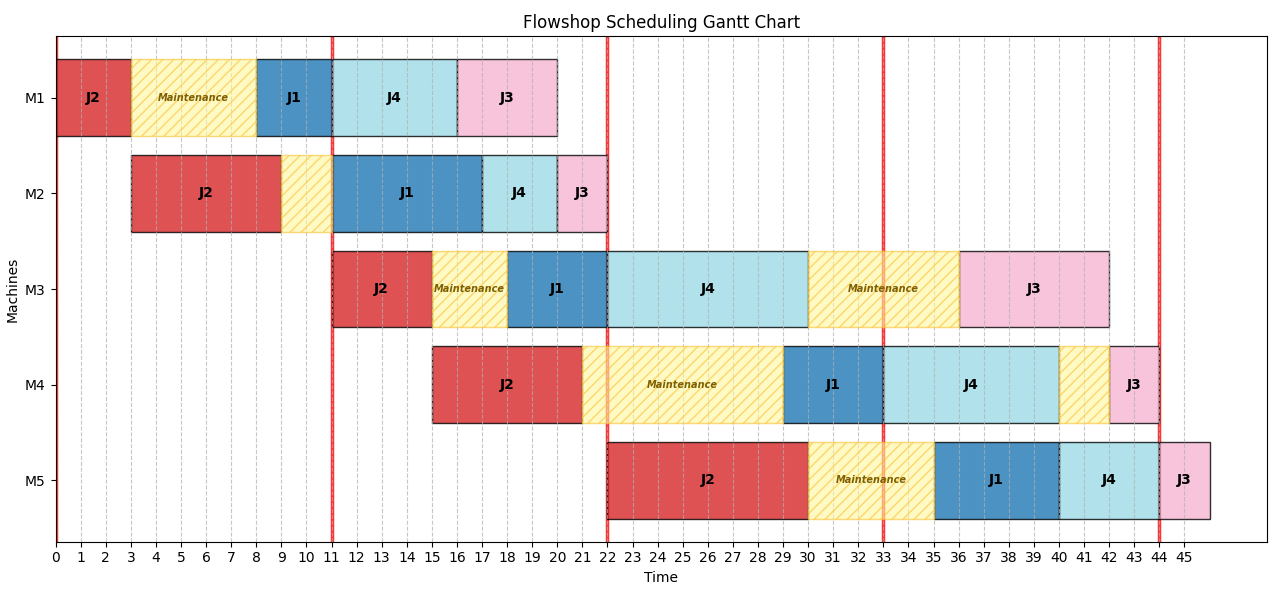
\includegraphics[width=0.95\textwidth]{images/gantt_chart.png}
    \caption{Representation of the solution to the problem with the Gantt Chart}
    \label{fig:gantt_chart}
\end{figure}
\chapter{Results}
\label{sec:intro_res}

To rigorously evaluate the performance of the metaheuristic, two distinct percentage gaps are computed:

\begin{itemize}
    \item \textbf{Gap vs Best:} Measures the deviation of the metaheuristic solution from the best feasible solution (Upper Bound) found by the exact algorithm.
    \begin{equation}
        \text{Gap}_{\text{Best}} (\%) = \frac{\text{Obj}_{\text{Meta}} - \text{Obj}_{\text{MIP}}}{\text{Obj}_{\text{MIP}}} \times 100
    \end{equation}
    
    \item \textbf{Gap vs LB (Worst-case Optimality Gap):} Measures the maximum possible deviation from the theoretical optimum, using the Lower Bound provided by the MIP solver. This metric is particularly useful for instances where the exact algorithm reaches the time limit without proving optimality.
    \begin{equation}
        \text{Gap}_{\text{LB}} (\%) = \frac{\text{Obj}_{\text{Meta}} - \text{LB}_{\text{MIP}}}{\text{LB}_{\text{MIP}}} \times 100
    \end{equation}
\end{itemize}

For instances solved to exact optimality within the time limit, the Best Objective and the Lower Bound coincide, rendering the two gap values identical.

All the results are shown in the \textbf{Table \ref{tab:results_comparison_lb}}.

\section[Table \ref{tab:results_comparison_lb} Analysis]{Table \ref{tab:results_comparison_lb} Analysis}

\subsection{Analysis of the obj. values}

\textbf{Histogram \ref{fig:obj_histogram_2}} and \textbf{Histogram \ref{fig:obj_histogram_1}} show the results in a histogram where  the number of the instance and its number of the jobs and of the machines is given. Here we can observe how the objective value of the MIP implementation at the beginning is equal to the metaheuristic value and the lower bound. These are the cases where the 300 seconds timer doesn't run out. As the number of jobs and machines increases, the MIP solver starts to reach the timer more frequently. So the solutions are found more rarely and, if found, are very far from the LB and the metaheuristic ones.

\begin{figure}
    \centering
    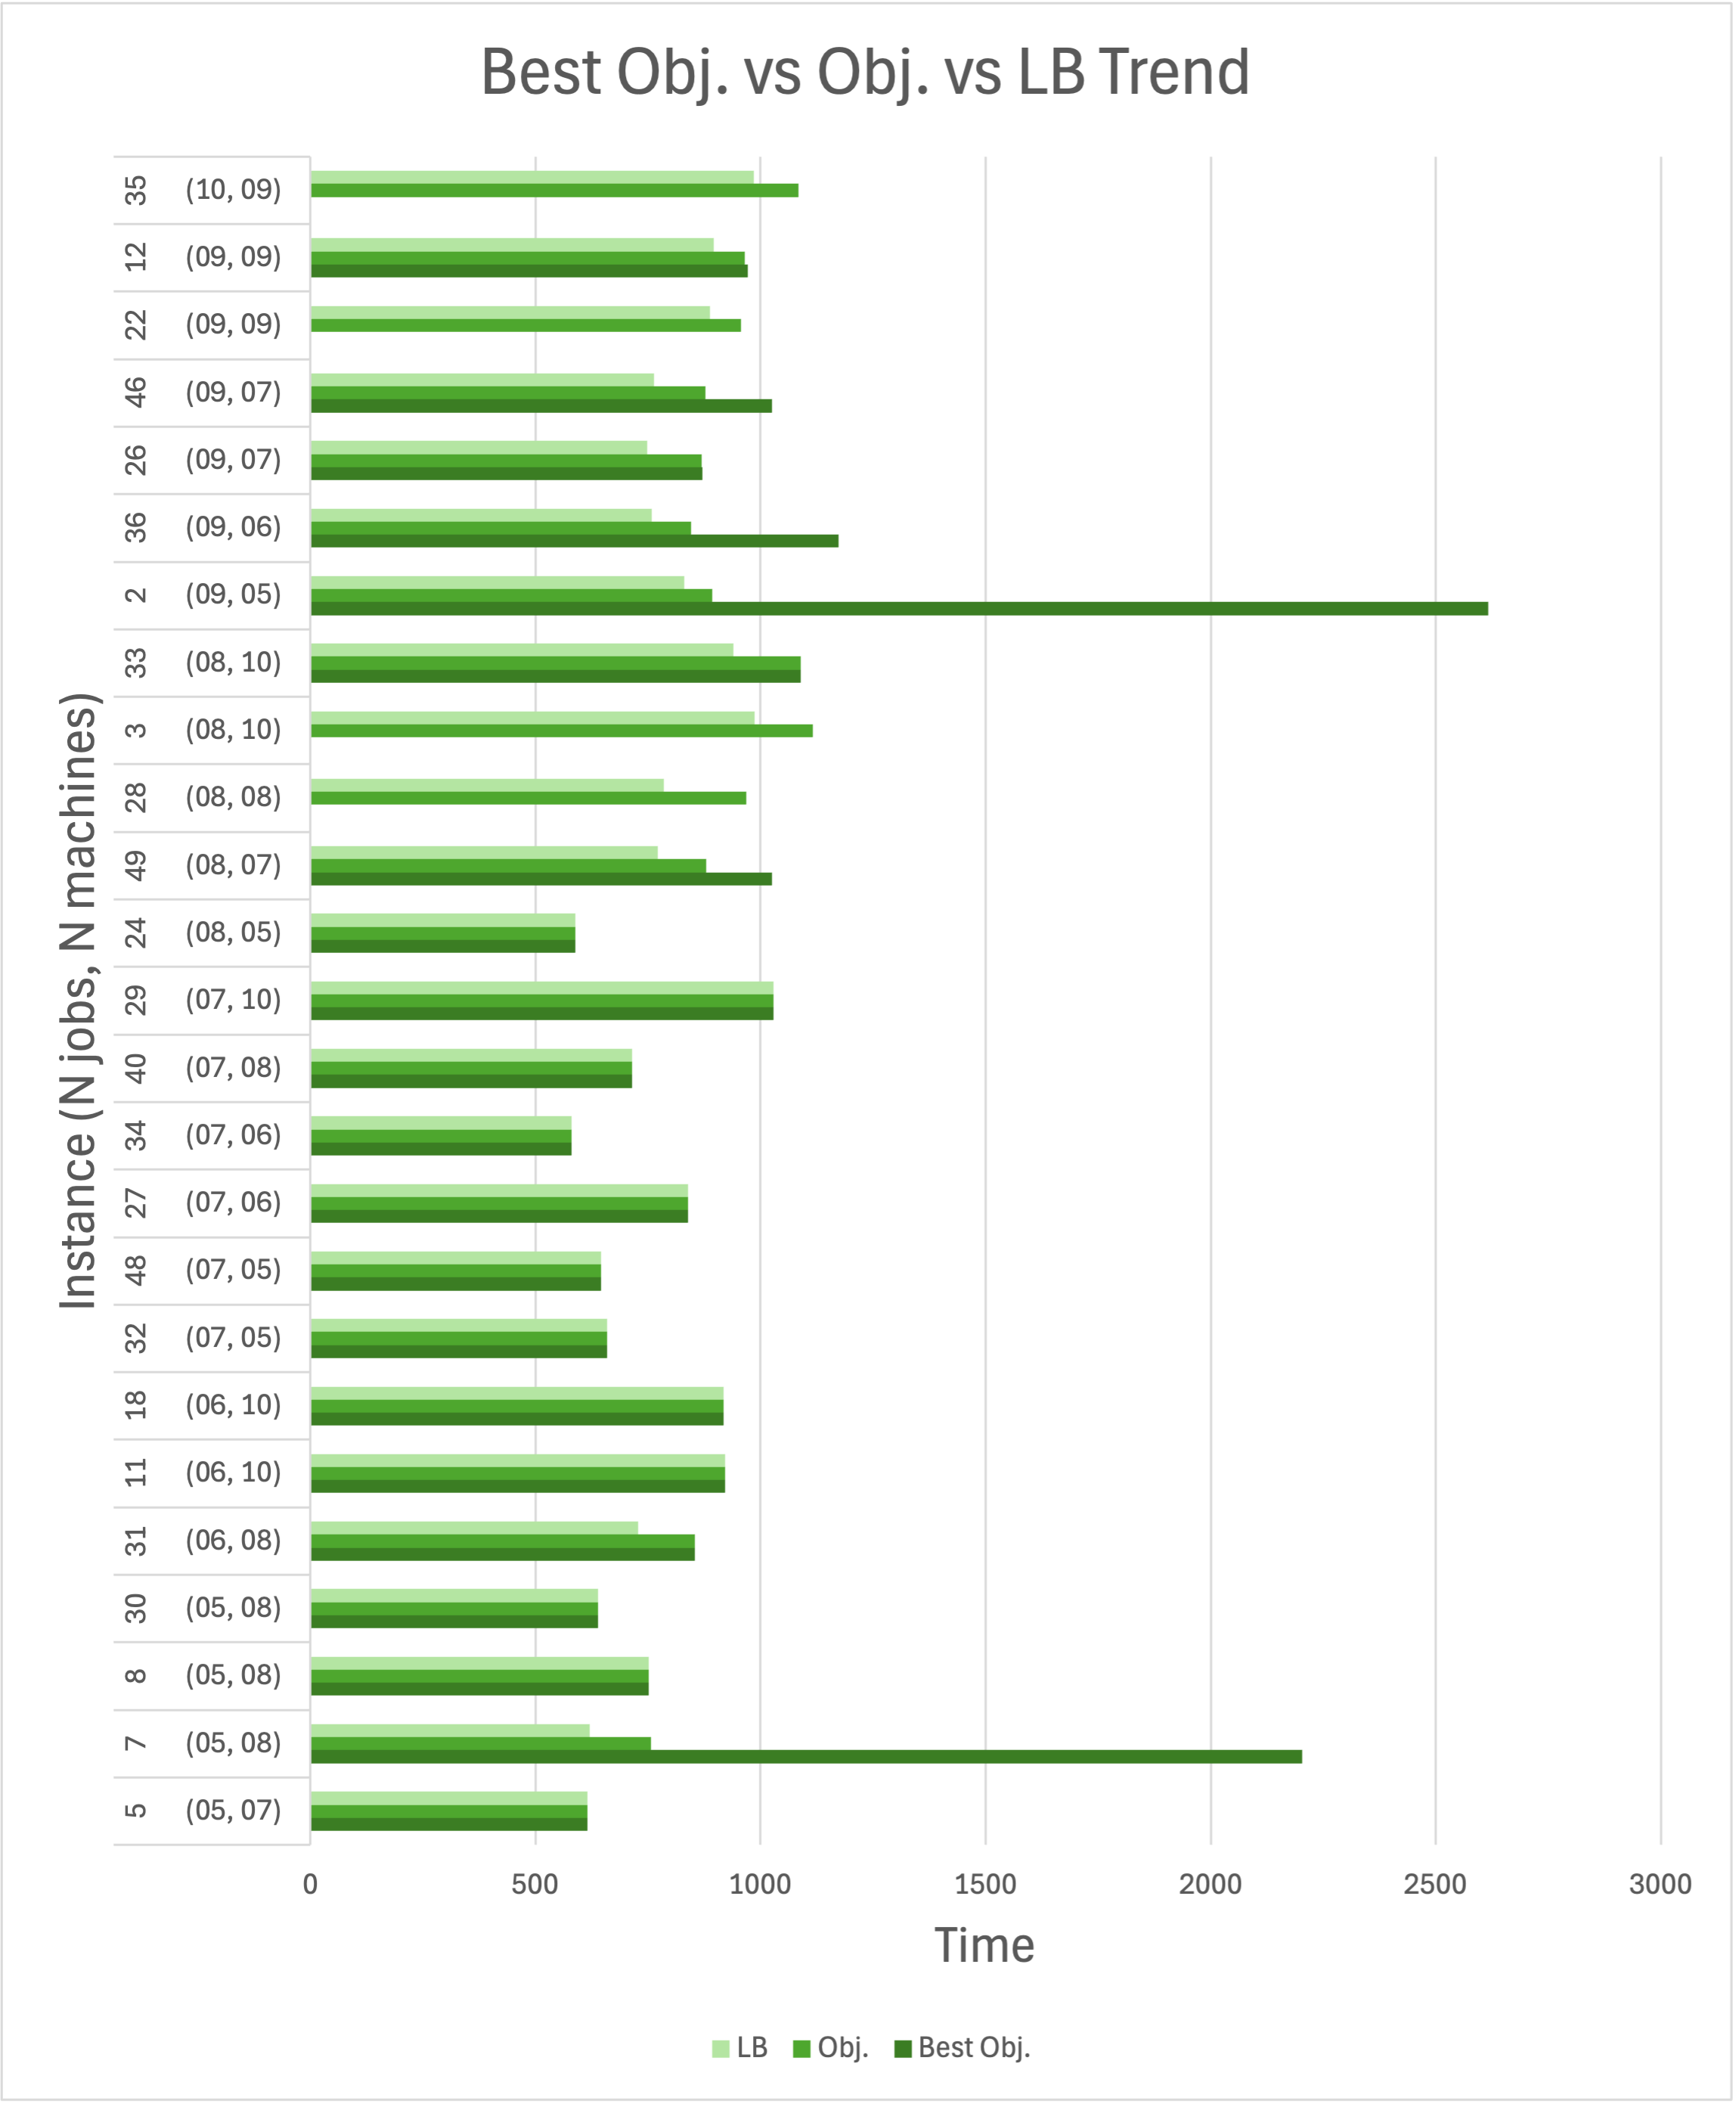
\includegraphics[width=0.95\textwidth]{images/obj_histogram_2.png}
    \caption{Representation of the objective values in an histogram}
    \label{fig:obj_histogram_2}
\end{figure}

\begin{figure}
    \centering
    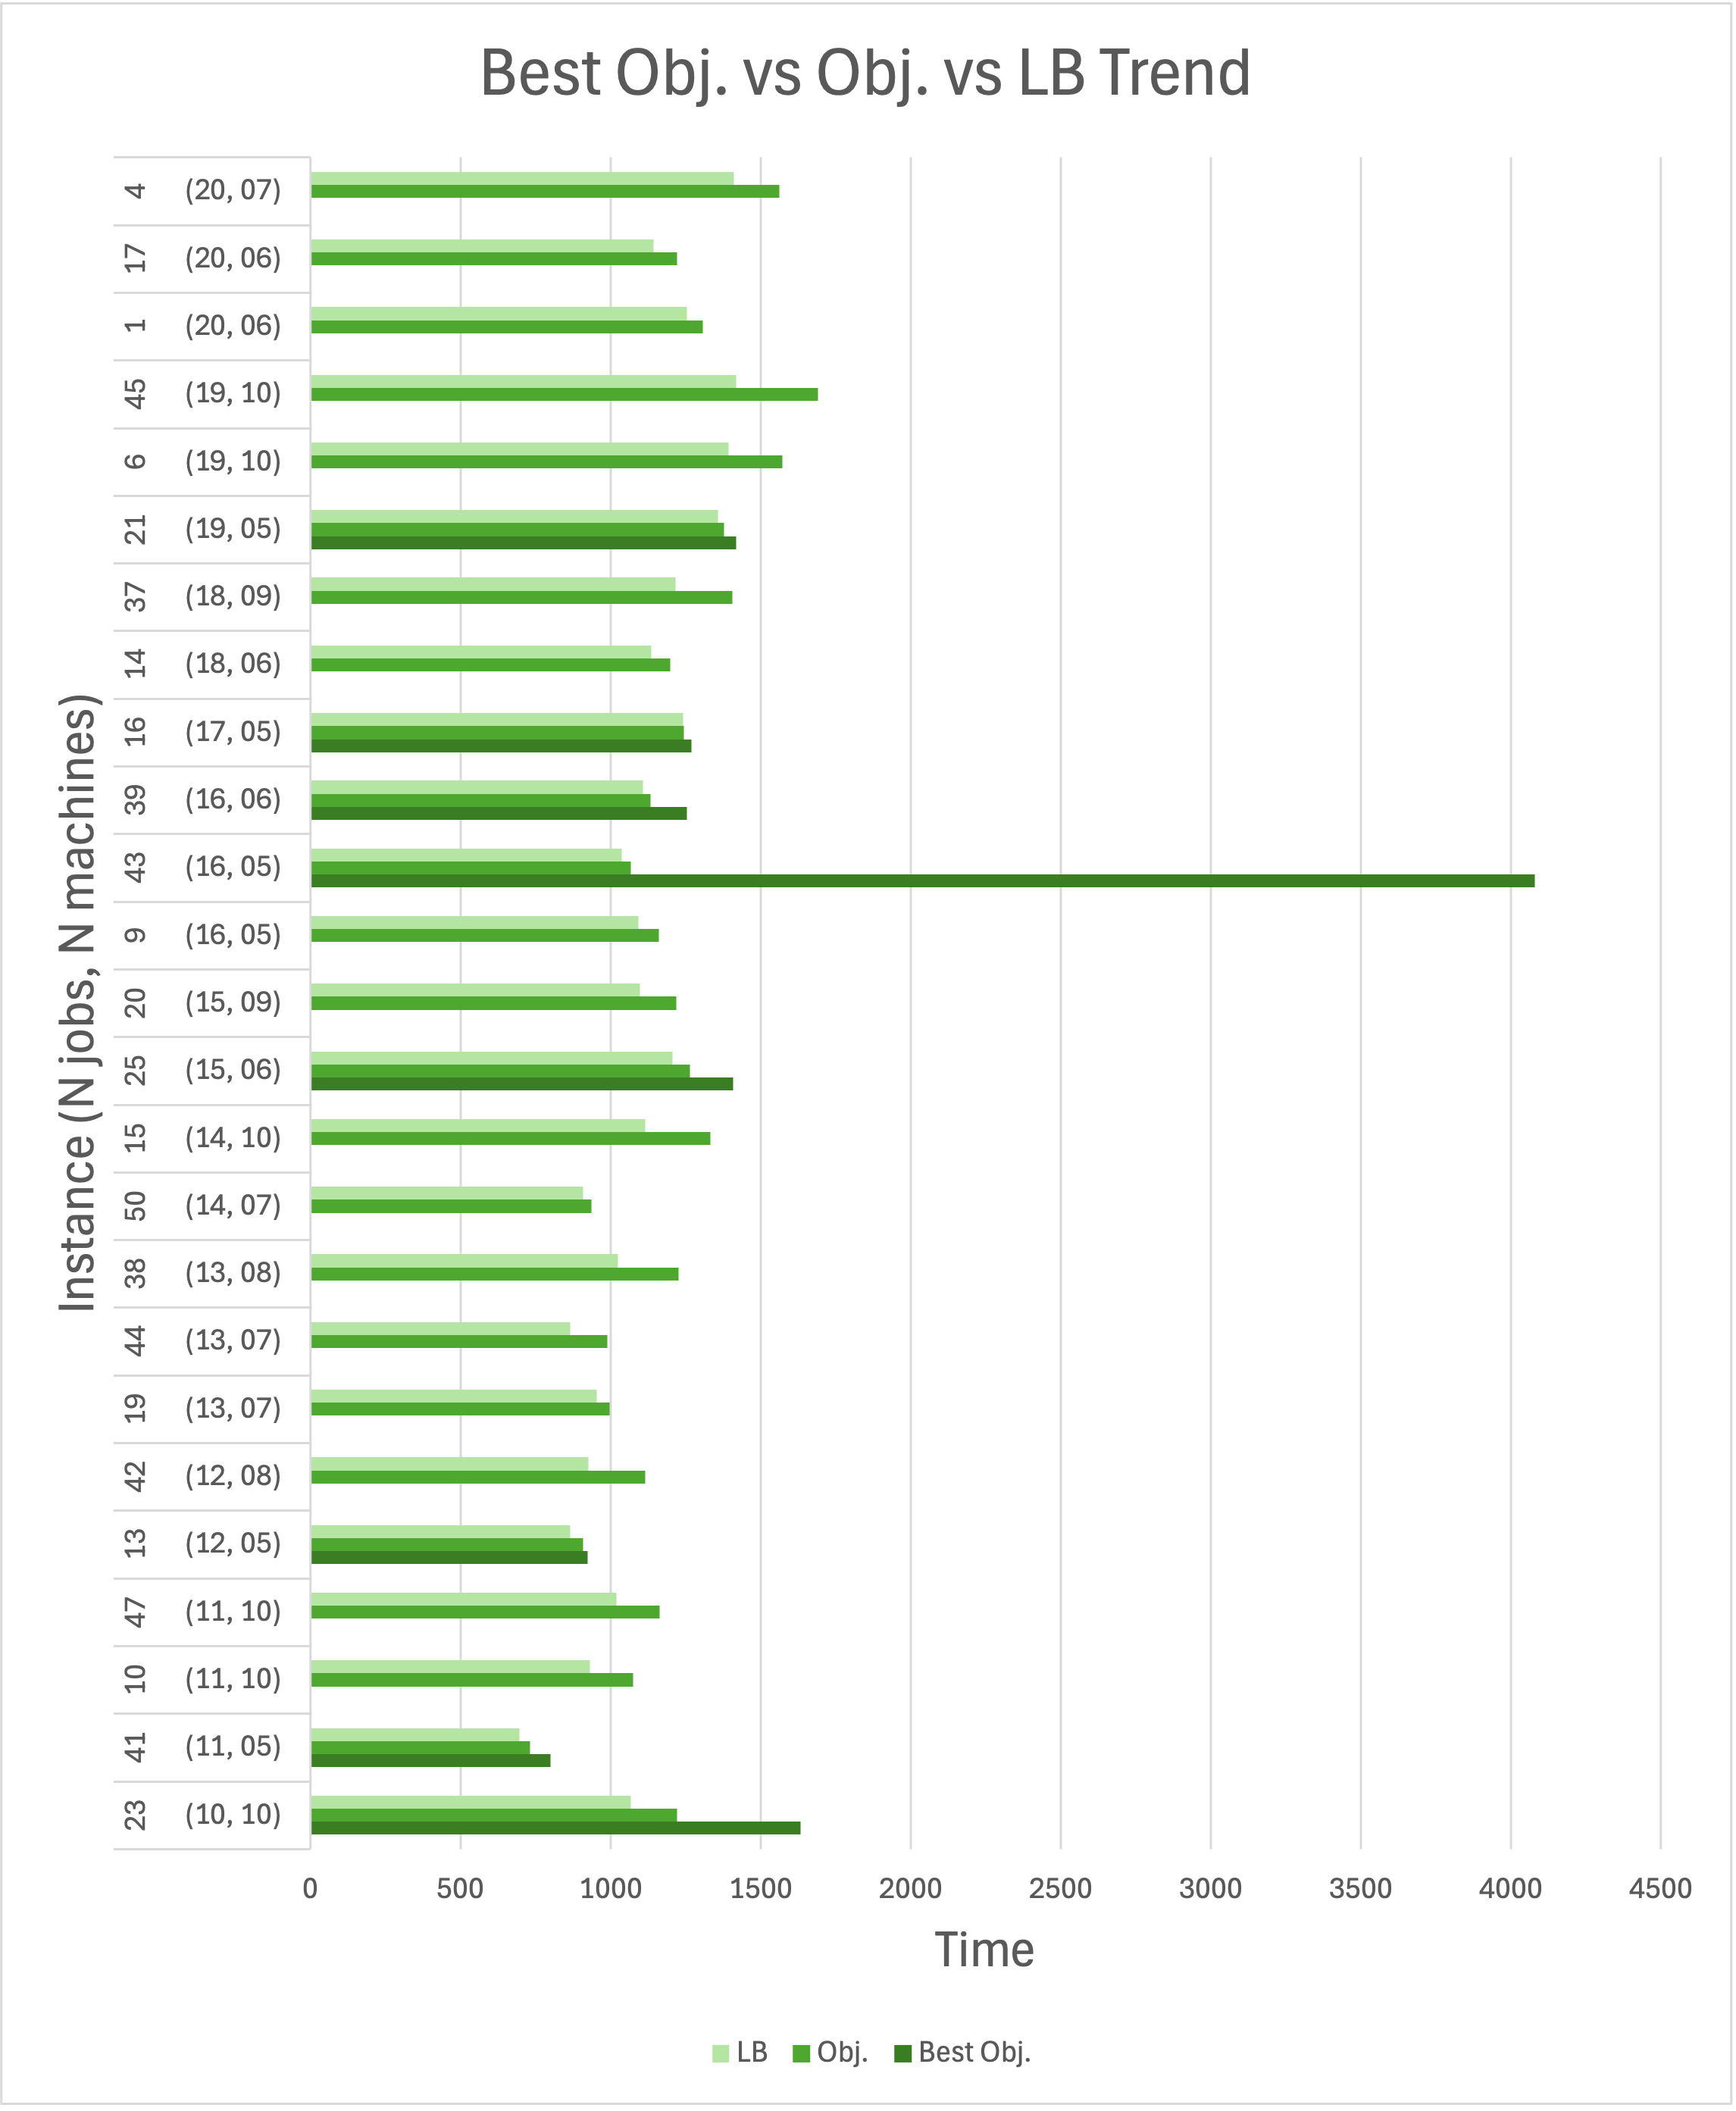
\includegraphics[width=0.95\textwidth]{images/obj_histogram_1.png}
    \caption{Representation of the objective values in an histogram}
    \label{fig:obj_histogram_1}
\end{figure}

The results show that the exact algorithm frequently reaches the maximum time, set on 300 seconds (exactly \textbf{74\%} of the times). That means that it gets lost analyzing all the branches of the search tree, sometimes not even finding a feasible solution. Indeed \textbf{42\%} of the times it doesn't find a solution and \textbf{34\%} of the times it finds a feasible solution. Instead the metaheuristic reaches the solution with a \textbf{100\%} success rate within few seconds.

Furthermore, when the MIP algorithm finds the best solution (within the 300 seconds, the \textbf{24\%} of the times) the objective value is always the same as the metaheuristic one implements.

The LB value moreover is always equal or less than the optimal solution and the metaheuristic solution. But the LB is just a minimal theoretical value that the function could reach if it was given more time. It is not the actual optimal solution. That's why the metaheuristic could have actually given the optimal solution without knowing it.

\subsection{Computational Time Analysis}

\textbf{Line graph \ref{fig:calculus_time}} shows an analysis on the computational time reached by the MIP solver and the metaheuristic.

\begin{figure}
    \centering
    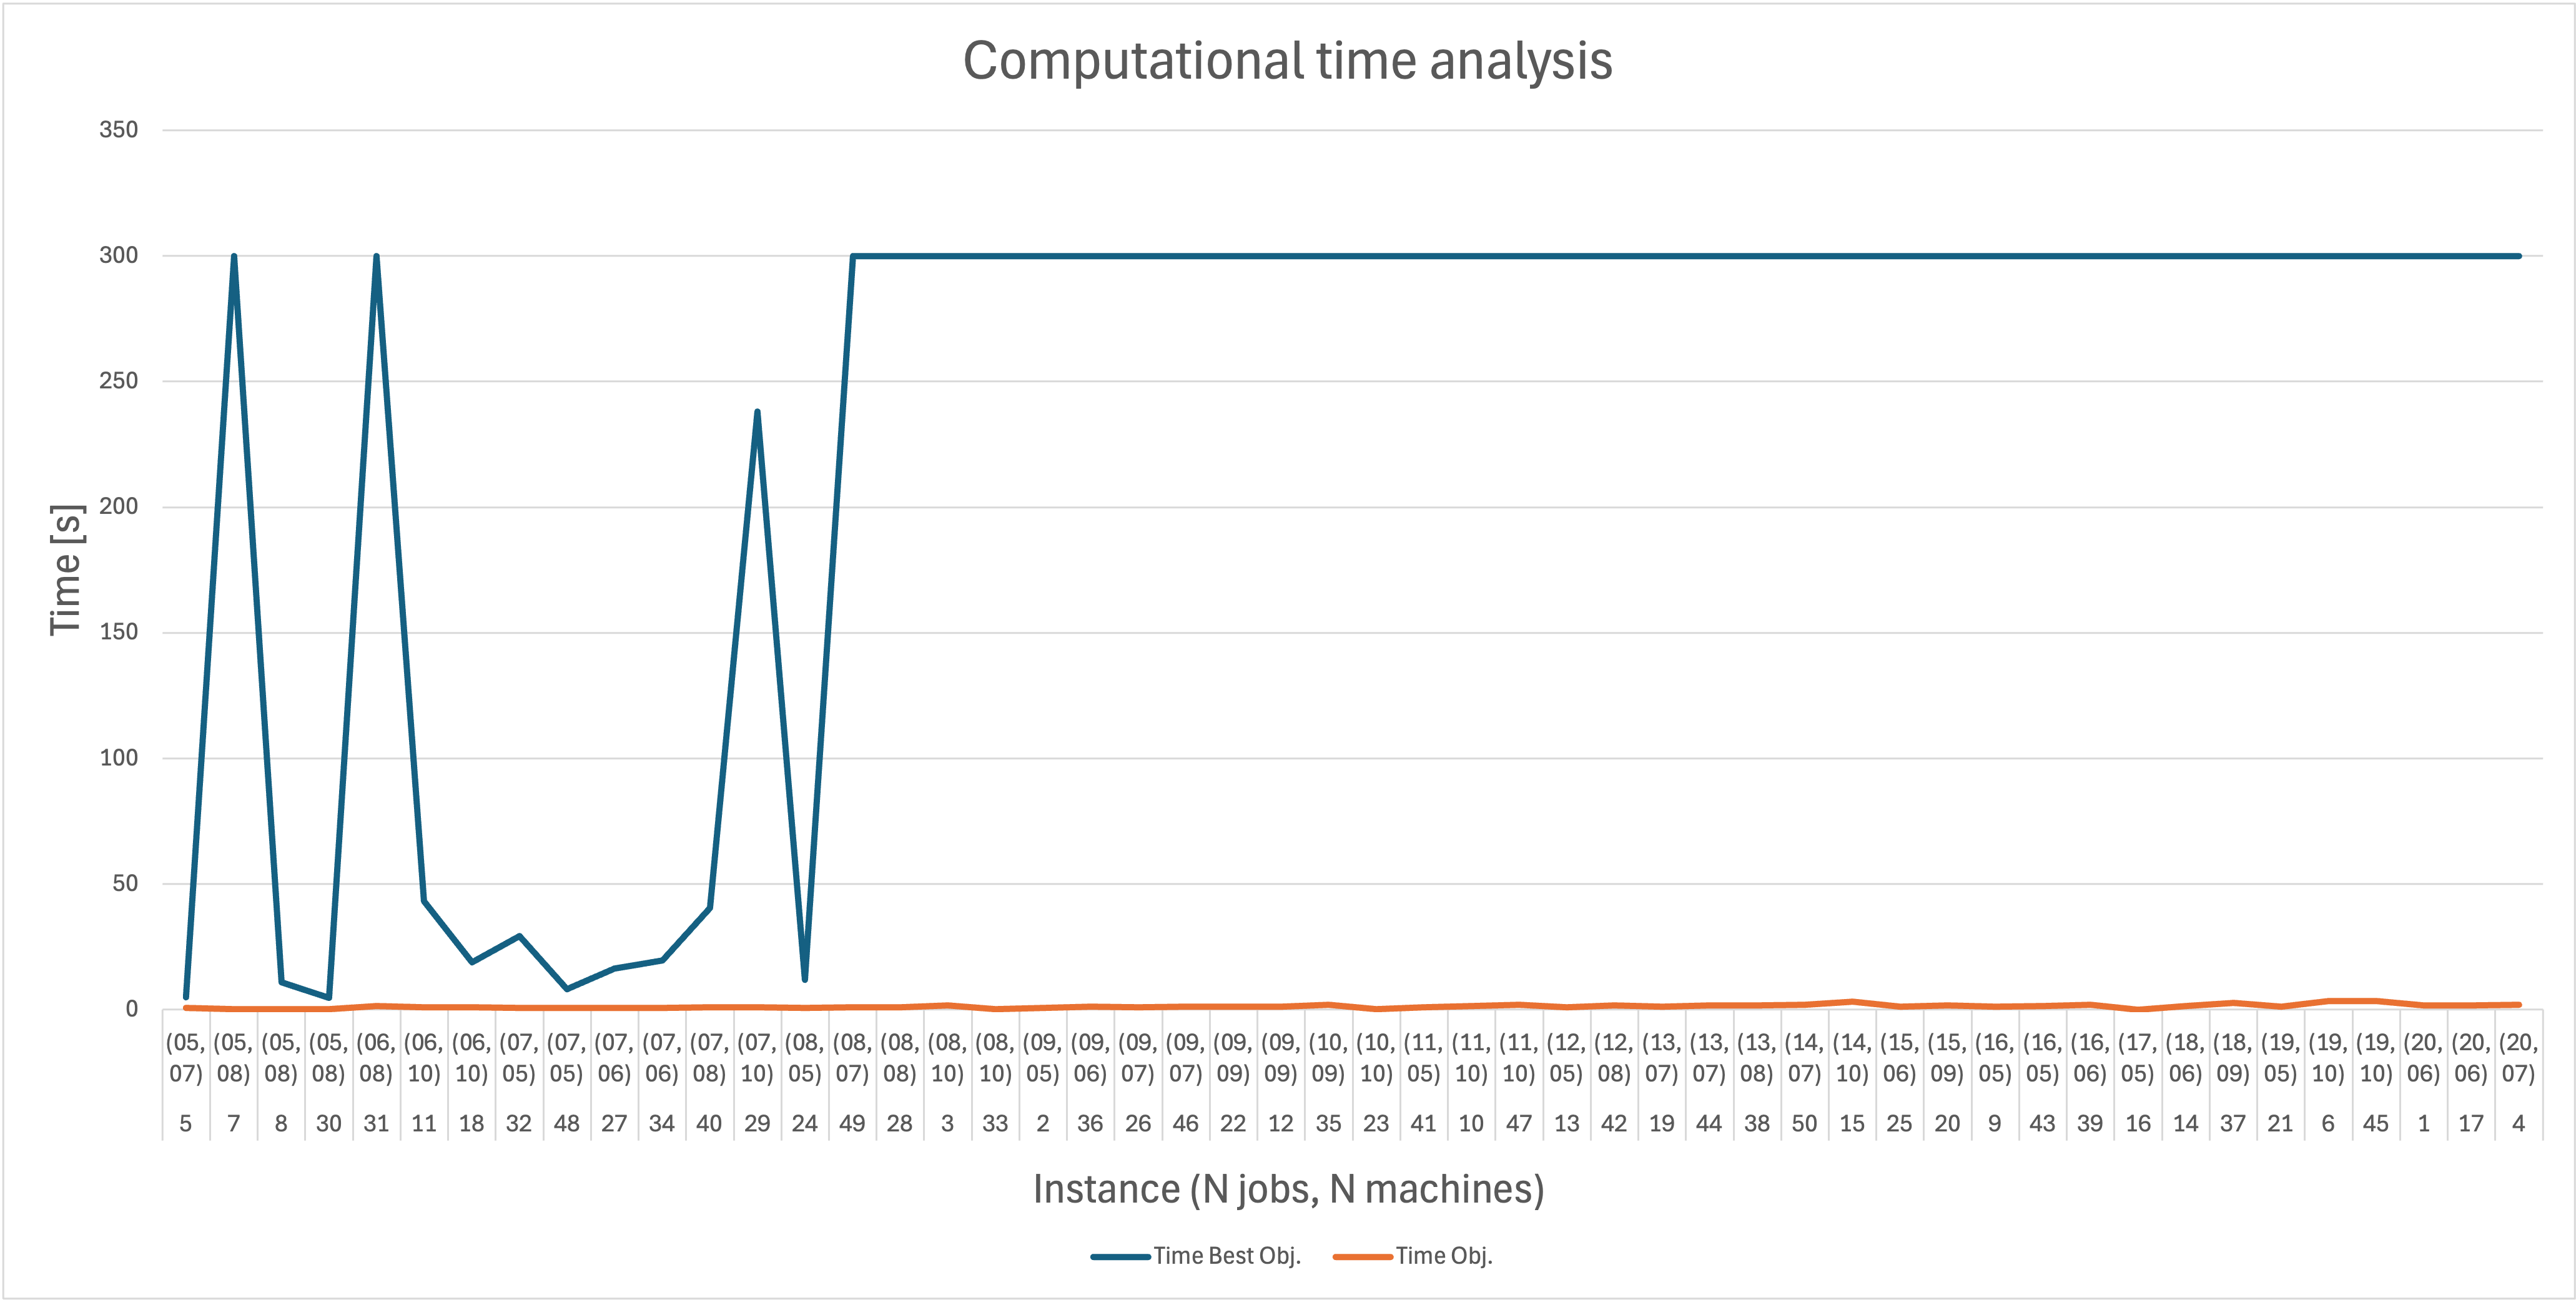
\includegraphics[width=0.95\textwidth]{images/calculus_time.png}
    \caption{Representation of the computational times in a line graph}
    \label{fig:calculus_time}
\end{figure}

It is clearly visible that, as the number of jobs ad of machines grows, the metaheuristic has a very small variation of the time spent while the MIP solver reaches the 300 seconds very rapidly.

\subsection{\% Gap Analysis}

\textbf{Line graph \ref{fig:perc_gap}} shows an analysis on the percentage gaps between the Obj. and the Best Obj. and between the LB and the Obj.

\begin{figure}
    \centering
    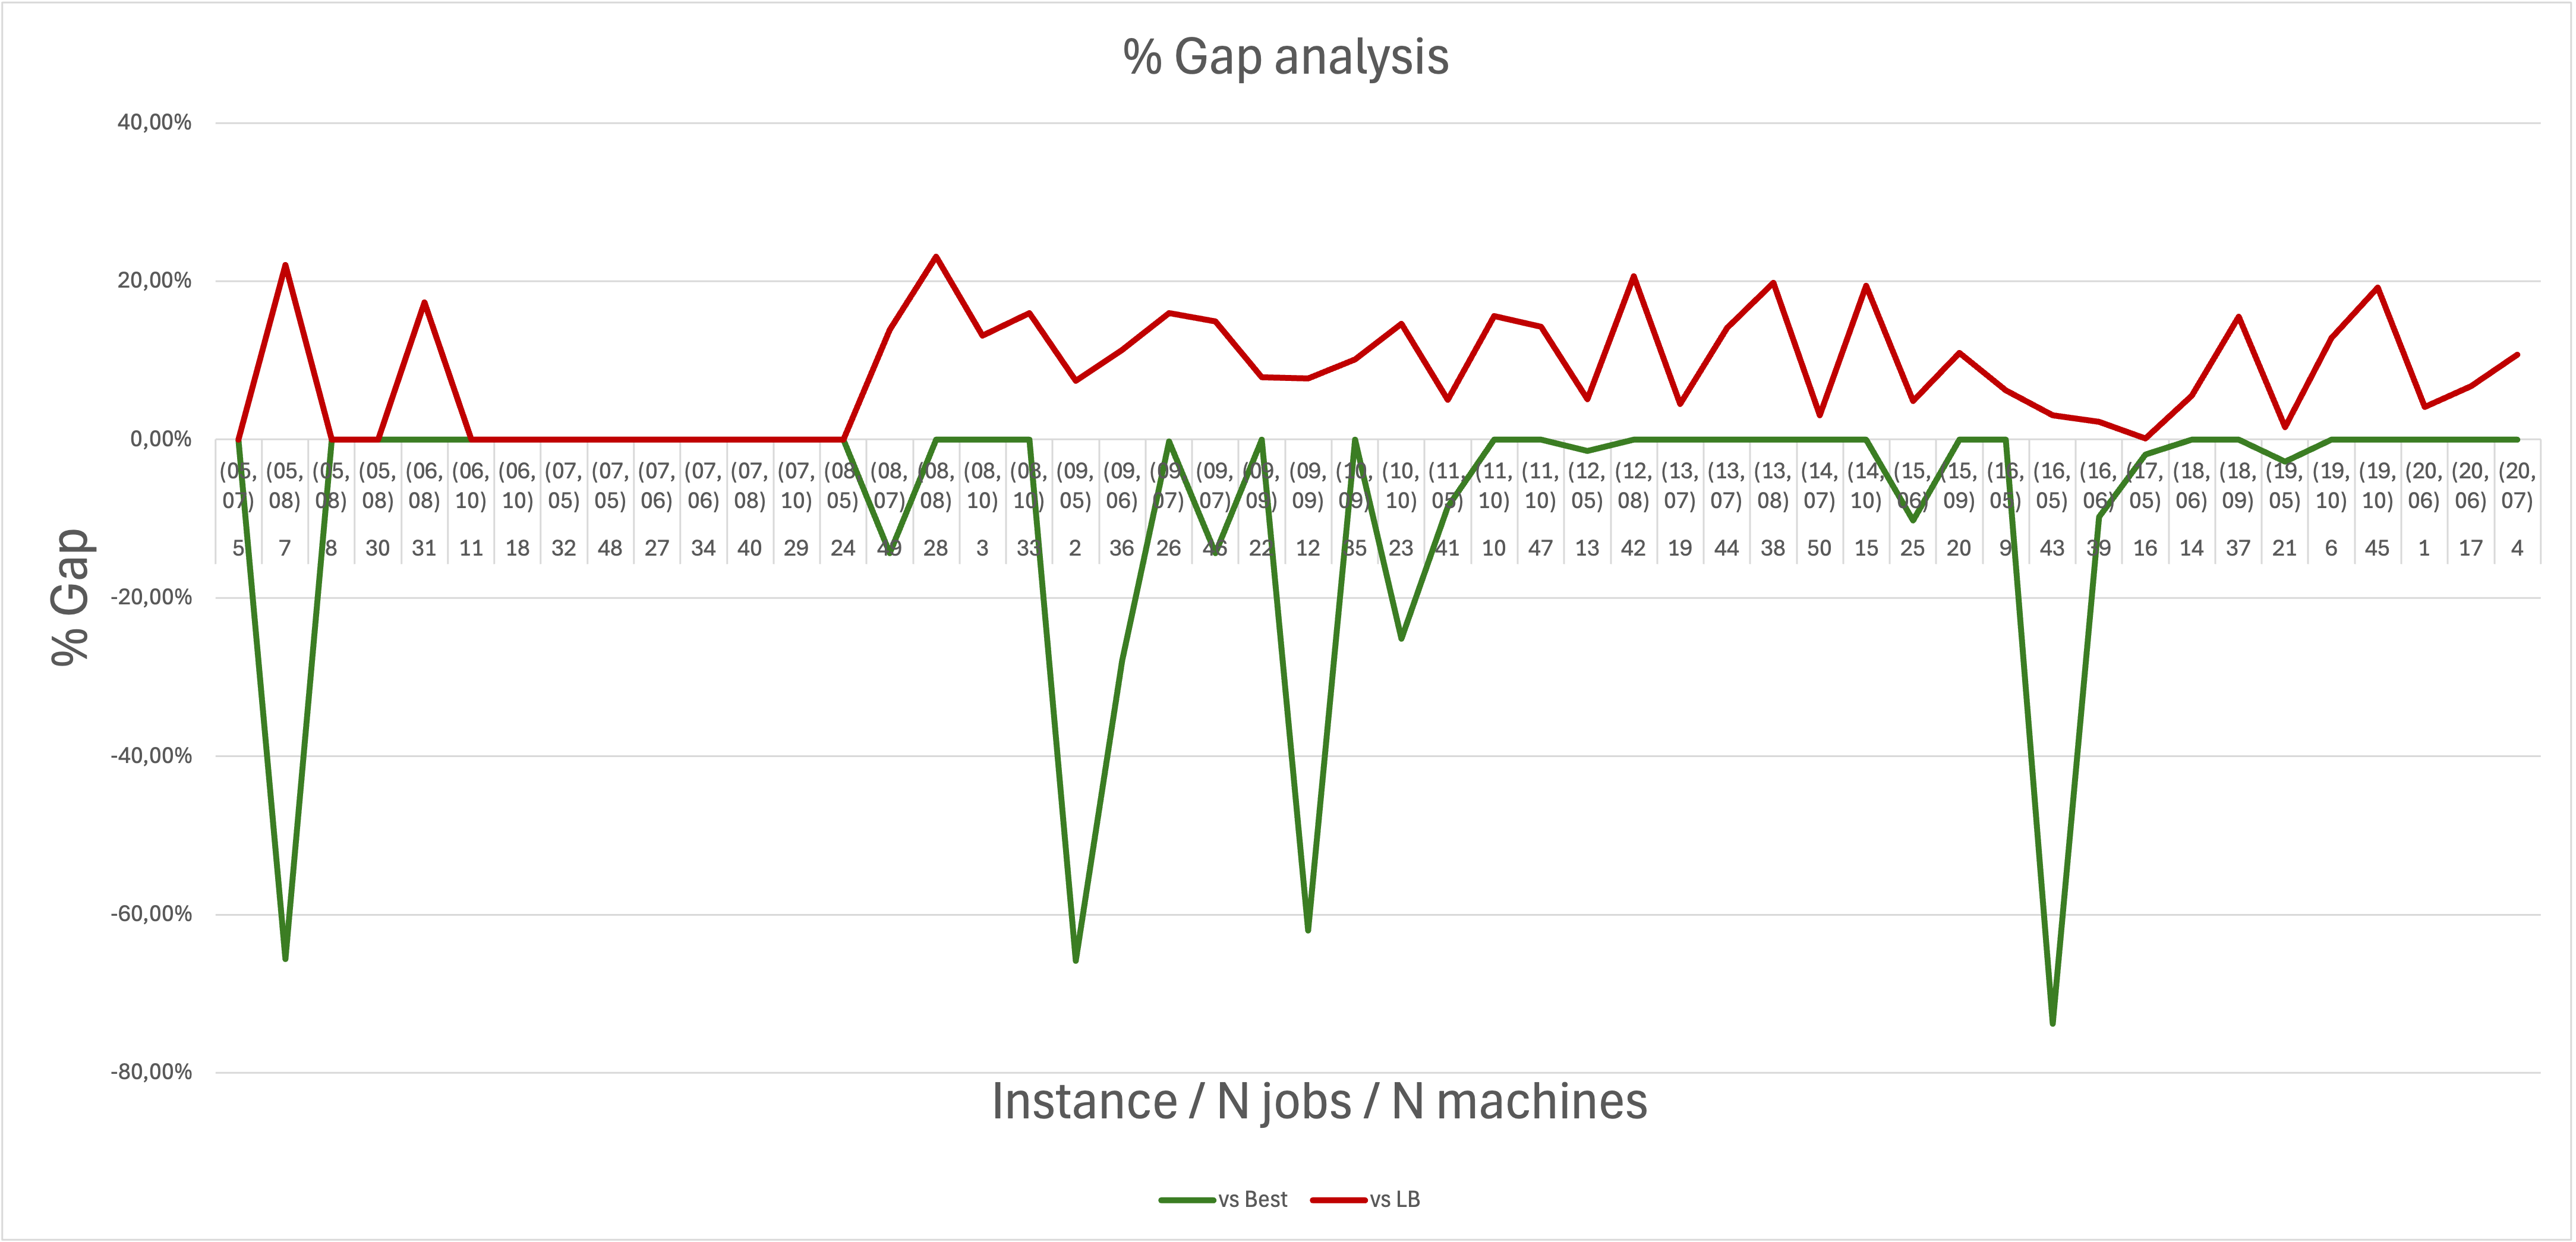
\includegraphics[width=0.95\textwidth]{images/perc_gap.png}
    \caption{Representation of the percentage gaps in a line graph}
    \label{fig:perc_gap}
\end{figure}

In the points where the lines coincide on the zero the MIP solver has reached the optimum in the 300 seconds timer. While where the "vs Best" reaches the zero value but the "vs LB" doesn't, represent the instances in which the MIP solver couldn't find a feasible solution.

The "vs LB" indicates that the percentage is always positive while the "vs Best" is always negative. That means that the LB value is always better or equals to the Obj. value of the metaheuristic while the Best Obj. value of the MIP solver is always equal or worse to the Obj. value of the metaheuristic.
\chapter{Conclusions}
\label{sec:intro_concl}

\section[Summary of the results and supremacy of the metaheuristic]{Summary of the results and supremacy of the metaheuristic}

As discussed in the previous chapter, the metaheuristic has surpassed the exact algorithm. In 74\% of the instances the MIP solver reached the timer limit and 42\% of the times failed to find a feasible solution, whereas 100\% of the time the metaheuristic could give a near optimal solution in just a few seconds. These results demonstrate that while exact solvers remain essential for finding theoretical lower bounds, they are highly impractical for more complex scenarios. Therefore, metaheuristics offer an optimal trade-off between computational time and solution quality for NP-hard problems.

Due to the factorial or exponential growth of the search space, increasing the time limit of the MIP solver yields diminishing returns. It would require an impractical amount of time to find the best solution and it may also be little better than the one the metaheuristic gives. The situation could be more manageable using fewer jobs and machines or less variable processing times. 

\section[Maintenance and industrial reality]{Maintenance and industrial reality}

Scheduling maintenance during idle times preserves company productivity without interrupting active processing phases. It means lengthening the useful life of the machines, keeping them in optimal condition and preventing unexpected breakdowns that would block the line. To make the model more applicable in real life, some enhancements could be made like considering the logistical times to move the semi-finished products between machines, the setup times of the machines or even the failure times (that even with great maintenance could happen). This could make the model a ``Digital Twin'' of the production scheduling.

\section[Decisional and sectorial flexibility]{Decisional and sectorial flexibility}

In \textbf{Figures \ref{fig:instance_40} and \ref{fig:instance_40mip}} it was pointed out how the same optimal solution could have different configurations regarding the starting or ending time of each production phase of each job or even the order of the jobs on the machines. This is a managerial advantage for the production manager that can choose the solution also based on secondary criteria without sacrificing the performance. Furthermore, the model has a timescale-agnostic approach that makes the algorithm flexible. It could be applied indifferently in high-frequency sectors, where times are measured in seconds, or in heavy industry, where one phase could span days or weeks.

In conclusion, this thesis demonstrate how developed models, like MIP solvers or the metaheuristics, can autonomously schedule (even in a few seconds) an entire production, solving modern manufacturing challenges and making the production systems more efficient and customizable through efficient code implementations. 

\appendix
% appendix
\chapter{Scripts}
\label{sec:appendix_galileo}

\lstdefinelanguage{JavaScript}{
  keywords={break, case, catch, continue, debugger, default, delete, do, else, finally, for, function, if, in, const, instanceof, new, return, switch, this, throw, try, typeof, var, void, while, with},
  morecomment=[l]{//},
  morecomment=[s]{/*}{*/},
  morestring=[b]',
  morestring=[b]",
  sensitive=true
}

\lstset{
  language=Python,
    basicstyle=\ttfamily\small,
    keywordstyle=\color{blue}\bfseries,
    stringstyle=\color{red},
    commentstyle=\color{green!60!black}\itshape,
    numbers=left,
    numberstyle=\tiny\color{gray},
    stepnumber=1,
    breaklines=true,
    frame=single,
}

\section{Data Generation Script}
\label{app:data_creation_script}
\lstinputlisting{scripts/creation_files.py}

\section{MIP implementation Script}
\label{app:mip_implementation_script}
\lstinputlisting{scripts/main.py}

\section{Simulated Annealing Script}
\label{app:simulated_annealing_script}
\lstinputlisting{scripts/simulated_annealing.py}

\section{Automation Script}
\label{app:automation_script}
\lstinputlisting{scripts/automation.py}

% lstlisting environment for direct inclusion
% \begin{lstlisting}[language=Python]
%     const test = test
% \end{lstlisting}

% for computational complexity
%$\mathcal{O}\left(n\log{n}\right)$

% verbatim
%\verb+numpy+

\DTLsetseparator{;}

\DTLloaddb{results}{scripts/results.csv}

\setlength{\tabcolsep}{3pt} 
{\footnotesize 

\begin{longtable}{l c c c c c c c}

    \caption{Computational results: Exact Algorithm vs. Metaheuristic.} \label{tab:results_comparison_lb} \\
    
    \toprule
    & \multicolumn{3}{c}{\textbf{Exact Alg. (MIP)}} & \multicolumn{2}{c}{\textbf{Metaheuristic}} & \multicolumn{2}{c}{\textbf{Gaps (\%)}} \\
    \cmidrule(lr){2-4} \cmidrule(lr){5-6} \cmidrule(lr){7-8}
    \textbf{Inst.} & \textbf{LB} & \textbf{Best Obj.} & \textbf{Time (s)} & \textbf{Obj.} & \textbf{Time (s)} & \textbf{vs Best} & \textbf{vs LB} \\
    \midrule
    \endfirsthead
    
    \multicolumn{8}{c}{{\bfseries \tablename\ \thetable{} -- Continuation from the previous page}} \\
    \toprule
    & \multicolumn{3}{c}{\textbf{Exact Alg. (MIP)}} & \multicolumn{2}{c}{\textbf{Metaheuristic}} & \multicolumn{2}{c}{\textbf{Gaps (\%)}} \\
    \cmidrule(lr){2-4} \cmidrule(lr){5-6} \cmidrule(lr){7-8}
    \textbf{Inst.} & \textbf{LB} & \textbf{Best Obj.} & \textbf{Time (s)} & \textbf{Obj.} & \textbf{Time (s)} & \textbf{vs Best} & \textbf{vs LB} \\
    \midrule
    \endhead
    
    \midrule
    \multicolumn{8}{r}{{Continues in the next page...}} \\
    \footnotemark
    \endfoot
    
    \bottomrule
    \multicolumn{8}{l}{\footnotesize * Best feasible solution found. Time limit reached.} \\
    \endlastfoot
    
    \noalign{\global\let\DTLcurrentline\relax}
    \DTLforeach{results}{
        \Inst=Instance,\LB=LB,\BestObj=Best Obj.,\TimeMIP=Time 1,\ObjMeta=Obj.,\TimeMeta=Time 2,\GapBest=vs Best,\GapLB=vs LB
    }{
        \detokenize\expandafter{\Inst} & \LB & \BestObj & \TimeMIP & \ObjMeta & \TimeMeta & \GapBest & \GapLB \\
    }

\end{longtable}
}

\end{document}

\clearpage
\mbox{}
\thispagestyle{plain} % Mantiene solo il numero di pagina, toglie le testatine in alto
\clearpage

\begingroup
  \renewcommand{\cleardoublepage}{\clearpage} % Forza LaTeX a non saltare pagine a destra
  \listoftables
  \listoffigures
\endgroup

% endnotes here if needed

\nocite{*}
\printbibliography

\end{document}
